\chapter{نتایج}
\label{ch:results}

همه اعداد این فصل در برابر آشکارسازی‌های راداری \lr{GFW} و با روش بخش~\ref{sec:evaluation}
به دست آمده‌اند. «همان خانه» قاعده اصلی است و «همسایه» قاعده آسان‌گیرتر.

\section{انتخاب پیکربندی روی اعتبارسنجی}
روی ۲۵ گذر اعتبارسنجی، \lr{CFAR} به \lr{F1} برابر \LRE{0٫807} (همسایه \LRE{0٫851}) رسید.
کاشی‌های ۲۵۶ پیکسلی از ۱۲۸ پیکسلی بهتر و سریع‌تر بودند و کاشی‌های کوچک، قله‌های تکراری
را دو برابر می‌کردند (آشکارسازی‌هایی در کمتر از ۱۰۰ متر از آشکارسازی دیگر: \LRE{8٫4}٪ با
کاشی ۱۲۸ و هم‌پوشانی ۳۲، \LRE{2٫8}٪ در پیکربندی برگزیده، \LRE{1٫3}٪ در \lr{CFAR}). آموزش
طولانی‌تر شناورهای بدون \lr{AIS} را از دست می‌داد: بازیابی آن‌ها از \LRE{0٫85} در دوره ۵ به
\LRE{0٫68} در دوره ۱۴ رسید. ازاین‌رو دوره ۵ با کاشی ۲۵۶ و آستانه \LRE{0٫60} برگزیده شد
(جدول~\ref{tab:validation} و شکل~\ref{fig:sweep}).

\begin{table}[htbp]
\centering
\small
\begin{adjustbox}{max width=\textwidth}
\begin{tabular}{lccccc}
\toprule
دوره آموزش & کاشی/هم‌پوشانی & آستانه & \lr{F1} & \lr{F1} همسایه & بازیابی بدون \lr{AIS} (همسایه) \\
\midrule
\LRE{5} & \LRE{256}/\LRE{64} & \LRE{0٫65} & \LRE{0٫831} & \LRE{0٫865} & \LRE{0٫798} \\
\LRE{5} & \LRE{256}/\LRE{64} & \LRE{0٫70} & \LRE{0٫825} & \LRE{0٫867} & \LRE{0٫746} \\
\textbf{\LRE{5}} & \textbf{\LRE{256}/\LRE{64}} & \textbf{\LRE{0٫60}} & \textbf{\LRE{0٫830}} & \textbf{\LRE{0٫862}} & \textbf{\LRE{0٫868}} \\
\LRE{5} & \LRE{256}/\LRE{64} & \LRE{0٫75} & \LRE{0٫819} & \LRE{0٫871} & \LRE{0٫667} \\
\LRE{8} & \LRE{256}/\LRE{64} & \LRE{0٫55} & \LRE{0٫823} & \LRE{0٫859} & \LRE{0٫789} \\
\LRE{5} & \LRE{256}/\LRE{64} & \LRE{0٫55} & \LRE{0٫824} & \LRE{0٫856} & \LRE{0٫877} \\
\bottomrule
\end{tabular}
\end{adjustbox}
\caption[انتخاب پیکربندی روی اعتبارسنجی]{انتخاب پیکربندی روی ۲۵ گذر اعتبارسنجی (هرگز روی آزمون): شش پیکربندی برتر به ترتیب میانگین \lr{F1} دو قاعده. از پیکربندی‌هایی که تا ۰٫۰۰۵ با بهترین فاصله داشتند، آنکه بازیابی بدون \lr{AIS} بیشتری داشت برگزیده شد (سطر پررنگ).}
\label{tab:validation}
\end{table}


\begin{figure}[htbp]
\centering
\begin{tikzpicture}
\begin{axis}[
  width=0.85\textwidth, height=6.5cm,
  xmin=0.05, xmax=0.9, ymin=0.2, ymax=1,
  xlabel={\rl{آستانه}}, ylabel={\rl{مقدار}},
  legend pos=south west, legend cell align=right,
  grid=major, grid style={gray!25},
]
\addplot[blue!70!black, thick, mark=*, mark size=1.2pt] table[x=threshold, y=f1] {../data/threshold_sweep.csv};
\addlegendentry{\rl{\lr{F1} همان خانه}}
\addplot[teal, thick, mark=square*, mark size=1.2pt] table[x=threshold, y=f1nb] {../data/threshold_sweep.csv};
\addlegendentry{\rl{\lr{F1} همسایه}}
\addplot[orange!80!black, thick, dashed, mark=triangle*, mark size=1.4pt] table[x=threshold, y=unmatched] {../data/threshold_sweep.csv};
\addlegendentry{\rl{بازیابی بدون \lr{AIS} (همان خانه)}}
\draw[red!70!black, densely dotted, thick] (axis cs:0.6,0.2) -- (axis cs:0.6,1);
\end{axis}
\end{tikzpicture}
\caption[اثر آستانه روی اعتبارسنجی]{اثر آستانه بر مدل نهایی (دوره ۵، کاشی ۲۵۶) روی گذرهای اعتبارسنجی. خط نقطه‌چین،
آستانه برگزیده \LRE{0٫60}. بالاتر بردن آستانه \lr{F1} را اندکی بالا می‌برد ولی شناورهای بدون
\lr{AIS} را از دست می‌دهد.}
\label{fig:sweep}
\end{figure}

\section{آزمون نگه‌داشته: سوگیری برچسب و رفع آن}
مقایسه اصلی از پیش روی ۴۰ گذر آزمون توافق شده بود و سپس به همه ۹۲ گذر آزمون گسترش یافت
(\testRefs{} آشکارسازی \lr{GFW}، \testRefsDark{} بدون \lr{AIS}). مدل نخست از \lr{CFAR} ضعیف‌تر
بود: روی ۴۰ گذر، \lr{F1} آن \LRE{0٫050} کمتر بود (بازه ۹۵٪: \LRE{0٫029} تا \LRE{0٫072}
کمتر). دلیل در ستون آخر جدول~\ref{tab:test40} پیداست: مدل نخست تنها نیمی از شناورهای بدون
\lr{AIS} را می‌یافت، چون برچسب‌های مثبتش فقط از شناورهای دارای \lr{AIS} آمده بود و
شناورهای بدون \lr{AIS} در داده آموزشی یا بی‌برچسب بودند یا نادیده گرفته می‌شدند. این همان
خطری است که یک سامانه پایش شناور تاریک نباید داشته باشد: آشکارسازی که از روی \lr{AIS}
آموخته، شناورهای بی‌\lr{AIS} را کمتر می‌بیند (شکل~\ref{fig:labelbias}).

مدل نهایی با افزودن \dataTrainDark{} آشکارسازی بدون \lr{AIS} \lr{GFW} به مثبت‌ها این سوگیری را
برطرف کرد. روی ۹۲ گذر آزمون \lr{F1} آن \testFOneModel{} در برابر \testFOneCfar{} برای \lr{CFAR}
بود؛ تفاضل \testDiff{} با بازه ۹۵٪ \testDiffCi{} معنادار است. با قاعده همسایه، تفاضل
\testDiffNb{} (بازه \testDiffNbCi) مرزی است (جدول~\ref{tab:test92}). برتری کوچک است و
باید چنین گزارش شود: مدل در این محدوده‌ها اندکی بهتر از \lr{CFAR} است، نه بسیار بهتر. روی
۱۹ گذر آزمونی که هیچ قاب هم‌گذرشان در آموزش یا اعتبارسنجی نبود، تفاضل \LRE{+0٫016} (بازه
\LRE{+0٫004} تا \LRE{+0٫032}) بود، پس برتری از آشنایی با گذرهای آموزشی نمی‌آید.

\begin{table}[htbp]
\centering
\small
\begin{adjustbox}{max width=\textwidth}
\begin{tabular}{lcccccc}
\toprule
آشکارساز & دقت & بازیابی & \lr{F1} & \lr{F1} همسایه & بازیابی با \lr{AIS} & بازیابی بدون \lr{AIS} \\
\midrule
\lr{CFAR} & \LRE{0٫710} & \LRE{0٫918} & \LRE{0٫800} & \LRE{0٫844} & \LRE{0٫930} & \LRE{0٫771} \\
مدل نخست (\lr{run 1}) & \LRE{0٫679} & \LRE{0٫838} & \LRE{0٫750} & \LRE{0٫807} & \LRE{0٫869} & \LRE{0٫477} \\
مدل نهایی (\lr{run 2}) & \LRE{0٫720} & \LRE{0٫931} & \LRE{0٫812} & \LRE{0٫853} & \LRE{0٫943} & \LRE{0٫787} \\
\bottomrule
\end{tabular}
\end{adjustbox}
\caption[آشکارسازها روی ۴۰ گذر آزمونِ توافق‌شده]{همان سنجش روی ۴۰ گذرِ آزمونی که مقایسه از پیش بر آن توافق شده بود.}
\label{tab:test40}
\end{table}

\begin{table}[htbp]
\centering
\small
\begin{adjustbox}{max width=\textwidth}
\begin{tabular}{lcccccc}
\toprule
آشکارساز & دقت & بازیابی & \lr{F1} & \lr{F1} همسایه & بازیابی با \lr{AIS} & بازیابی بدون \lr{AIS} \\
\midrule
\lr{CFAR} & \LRE{0٫716} & \LRE{0٫927} & \LRE{0٫808} & \LRE{0٫848} & \LRE{0٫938} & \LRE{0٫768} \\
مدل نخست (\lr{run 1}) & \LRE{0٫688} & \LRE{0٫855} & \LRE{0٫763} & \LRE{0٫820} & \LRE{0٫879} & \LRE{0٫504} \\
مدل نهایی (\lr{run 2}) & \LRE{0٫723} & \LRE{0٫938} & \LRE{0٫817} & \LRE{0٫854} & \LRE{0٫946} & \LRE{0٫813} \\
\bottomrule
\end{tabular}
\end{adjustbox}
\caption[آشکارسازها روی ۹۲ گذر آزمون]{آشکارسازها در برابر \lr{GFW} روی ۹۲ گذر-محدوده آزمون (قاعده «همان خانه» برای دقت، بازیابی و \lr{F1}؛ ستون «\lr{F1} همسایه» با خانه‌های همسایه).}
\label{tab:test92}
\end{table}


\begin{figure}[htbp]
\centering
\begin{tikzpicture}
\begin{axis}[
  width=0.75\textwidth, height=6cm,
  ybar, bar width=16pt, ymin=0, ymax=1.05,
  symbolic x coords={CFAR,run1,run2}, xtick=data,
  xticklabels={\lr{CFAR}, \rl{مدل نخست}, \rl{مدل نهایی}},
  ylabel={\rl{بازیابی (همان خانه)}},
  legend style={at={(0.5,1.03)}, anchor=south, legend columns=2},
  nodes near coords, nodes near coords style={font=\scriptsize},
  every node near coord/.append style={/pgf/number format/fixed, /pgf/number format/precision=2},
  enlarge x limits=0.25,
]
\addplot[fill=blue!45] table[x=detector, y=matched] {../data/label_bias.csv};
\addlegendentry{\rl{با \lr{AIS}}}
\addplot[fill=orange!65] table[x=detector, y=unmatched] {../data/label_bias.csv};
\addlegendentry{\rl{بدون \lr{AIS}}}
\end{axis}
\end{tikzpicture}
\caption[سوگیری برچسب]{سوگیری برچسب: بازیابی شناورهای با و بدون \lr{AIS} روی ۹۲ گذر آزمون. مدل نخست که
تنها از شناورهای دارای \lr{AIS} آموخته بود، نیمی از شناورهای بدون \lr{AIS} را از دست می‌داد.}
\label{fig:labelbias}
\end{figure}

برتری مدل در همه محدوده‌ها یکسان نیست (جدول~\ref{tab:areas-uae}): در آبراه هرمز و
راس‌الخیمه مدل آشکارا بهتر است، در فجیره برابر و در خورفکان اندکی ضعیف‌تر. همان‌طور که در
بخش بعد دیده می‌شود، بخشی از برتری مدل در محدوده‌های ساحلی به هشدارهای نادرست بیشتر
\lr{CFAR} نزدیک ساحل برمی‌گردد.

\begin{table}[htbp]
\centering
\small
\begin{adjustbox}{max width=\textwidth}
\begin{tabular}{lccccc}
\toprule
محدوده & آشکارسازی \lr{GFW} & \lr{F1} \lr{CFAR} & \lr{F1} مدل & همسایه \lr{CFAR} & همسایه مدل \\
\midrule
فجیره & \LRE{1٬455} & \LRE{0٫840} & \LRE{0٫839} & \LRE{0٫873} & \LRE{0٫873} \\
آبراه هرمز & \LRE{265} & \LRE{0٫806} & \LRE{0٫859} & \LRE{0٫860} & \LRE{0٫918} \\
خورفکان & \LRE{1٬066} & \LRE{0٫799} & \LRE{0٫794} & \LRE{0٫832} & \LRE{0٫820} \\
راس‌الخیمه & \LRE{244} & \LRE{0٫749} & \LRE{0٫807} & \LRE{0٫813} & \LRE{0٫859} \\
شارجه / دبی & \LRE{870} & \LRE{0٫782} & \LRE{0٫799} & \LRE{0٫832} & \LRE{0٫849} \\
\bottomrule
\end{tabular}
\end{adjustbox}
\caption[نتایج هر محدوده امارات]{مدل نهایی و \lr{CFAR} در هر محدوده مطالعاتی امارات (۹۲ گذر آزمون).}
\label{tab:areas-uae}
\end{table}


\section{تعمیم به زمان، ماهواره‌های تازه و ساحل ایران}
مدل نهایی منجمد شد و بدون هیچ بازتنظیمی روی چهار مجموعه دیگر سنجیده شد
(جدول~\ref{tab:generalisation} و شکل~\ref{fig:generalisation}).

\textbf{زمان دیگر:} روی ۲۰ گذر \lr{Sentinel-1A} نیمه نخست ۲۰۲۶ مدل و \lr{CFAR} هم‌تراز بودند
(تفاضل \genUaeEarlyStdDiff{}، بازه \genUaeEarlyStdCi).

\textbf{ماهواره‌های تازه:} روی ۴۷ گذر \lr{Sentinel-1C/1D} سپتامبر ۲۰۲۶ هر دو آشکارساز
\lr{F1} کمتری داشتند (مدل \genUaeNewStdModel{}، \lr{CFAR} \genUaeNewStdCfar) و باز هم‌تراز
بودند. افت برای هر دو یکسان است و از مرجع می‌آید، نه از مدل: سطح بازتاب دریا در تصاویر تازه
تغییری نکرده بود، ولی \lr{GFW} روی این ماهواره‌ها کم‌پشت‌تر است و \LRE{43}٪ آشکارسازی‌هایش
بدون \lr{AIS} است؛ بیشتر این سهم از یک خطای \lr{GFW} می‌آید: گذرِ حدود ساعت \LRE{02:07} به وقت
جهانی بر فجیره و خورفکان از ۲ اکتبر ۲۰۲۵ هیچ تطبیق \lr{AIS} ندارد، در حالی که حضور \lr{AIS}
در همان ساعت‌ها کامل است؛ بدون این گذر، سهم بدون \lr{AIS} \LRE{20}٪ است.

\begin{table}[htbp]
\centering
\small
\begin{adjustbox}{max width=\textwidth}
\begin{tabular}{lccccccc}
\toprule
مجموعه & امتیازدهی & گذر & آشکارسازی \lr{GFW} & \lr{F1} \lr{CFAR} & \lr{F1} مدل & مدل منهای \lr{CFAR} & بازه ۹۵٪ \\
\midrule
امارات، آزمون & استاندارد & \LRE{92} & \LRE{3٬900} & \LRE{0٫808} & \LRE{0٫817} & \LRE{+0٫009} & \LRE{+0٫002} تا \LRE{+0٫016} \\
 & دور از ساحل & \LRE{92} & \LRE{3٬900} & \LRE{0٫812} & \LRE{0٫817} & \LRE{+0٫005} & \LRE{−0٫001} تا \LRE{+0٫013} \\
امارات، \lr{S1A} ۲۰۲۶ & استاندارد & \LRE{20} & \LRE{854} & \LRE{0٫833} & \LRE{0٫827} & \LRE{−0٫006} & \LRE{−0٫022} تا \LRE{+0٫008} \\
 & دور از ساحل & \LRE{20} & \LRE{854} & \LRE{0٫835} & \LRE{0٫827} & \LRE{−0٫008} & \LRE{−0٫023} تا \LRE{+0٫006} \\
امارات، \lr{S1C/D} & استاندارد & \LRE{47} & \LRE{1٬899} & \LRE{0٫718} & \LRE{0٫721} & \LRE{+0٫003} & \LRE{−0٫006} تا \LRE{+0٫014} \\
 & دور از ساحل & \LRE{47} & \LRE{1٬893} & \LRE{0٫722} & \LRE{0٫721} & \LRE{0٫000} & \LRE{−0٫009} تا \LRE{+0٫011} \\
ایران، \lr{S1A} & استاندارد & \LRE{79} & \LRE{1٬184} & \LRE{0٫674} & \LRE{0٫781} & \LRE{+0٫108} & \LRE{+0٫085} تا \LRE{+0٫137} \\
 & دور از ساحل & \LRE{79} & \LRE{1٬178} & \LRE{0٫780} & \LRE{0٫795} & \LRE{+0٫015} & \LRE{+0٫002} تا \LRE{+0٫030} \\
ایران، \lr{S1C/D} & استاندارد & \LRE{62} & \LRE{517} & \LRE{0٫491} & \LRE{0٫644} & \LRE{+0٫152} & \LRE{+0٫113} تا \LRE{+0٫207} \\
 & دور از ساحل & \LRE{62} & \LRE{503} & \LRE{0٫631} & \LRE{0٫652} & \LRE{+0٫022} & \LRE{+0٫004} تا \LRE{+0٫047} \\
\bottomrule
\end{tabular}
\end{adjustbox}
\caption[تعمیم به زمان، ماهواره‌های تازه و ساحل ایران]{تعمیم مدل نهایی (منجمد) به زمان، ماهواره‌های تازه و منطقه تازه، در برابر \lr{GFW} (قاعده «همان خانه»). آزمون و ایران \lr{S1A}: \lr{Sentinel-1A} ۲۰۲۴–۲۰۲۵؛ \lr{S1A} ۲۰۲۶: نیمه نخست ۲۰۲۶؛ \lr{S1C/D}: \lr{Sentinel-1C/1D} سپتامبر ۲۰۲۶. «دور از ساحل» تنها خانه‌های بیش از ۱ کیلومتر از خشکی را می‌شمارد، که \lr{GFW} در آن‌ها آشکارسازی گزارش می‌کند. بازه‌ها با بوت‌استرپ جفتی روی گذرها.}
\label{tab:generalisation}
\end{table}


\textbf{منطقه دیگر:} روی ساحل ایران، با امتیازدهی استاندارد، مدل با فاصله زیادی از
\lr{CFAR} جلوتر است (\lr{S1A}: \genIranTestStdDiff{}، بازه \genIranTestStdCi). اما این برتری
بیشتر از نوار نزدیک ساحل می‌آید: \lr{GFW} در نوار یک‌کیلومتری ساحل آشکارسازی گزارش نمی‌کند، و
در این نوار \lr{CFAR} \LRE{440} هشدار نادرست داشت و مدل \LRE{51}. با شمردن تنها خانه‌های
دورتر از ۱ کیلومتر، برتری مدل کوچک اما معنادار می‌ماند: \genIranTestFarDiff{} (بازه
\genIranTestFarCi) روی \lr{S1A} و \genIranNewFarDiff{} (بازه \genIranNewFarCi) روی
\lr{S1C/S1D}. \lr{F1} مدل دور از ساحل \genIranTestFarModel{} بود، نزدیک به \genUaeTestStdModel{}
آزمون امارات. در ساحل ایران \LRE{70}٪ آشکارسازی‌های \lr{GFW} بدون \lr{AIS} است و مدل
\LRE{0٫93} آن‌ها را یافت. در امتیازدهی دور از ساحل امارات، برتری مدل به \genUaeTestFarDiff{}
(بازه \genUaeTestFarCi) کاهش می‌یابد و دیگر معنادار نیست؛ پس در هر دو منطقه بخشی از برتری مدل، کنار گذاشتن
بهتر ساحل است.

\begin{figure}[htbp]
\centering
\begin{tikzpicture}
\begin{axis}[
  width=0.95\textwidth, height=6.5cm,
  xmin=-0.6, xmax=4.6, ymin=-0.04, ymax=0.22,
  xtick={0,1,2,3,4},
  xticklabels={\rl{آزمون امارات}, \rl{امارات ۲۰۲۶}, \rl{امارات \lr{S1C/D}}, \rl{ایران \lr{S1A}}, \rl{ایران \lr{S1C/D}}},
  tick label style={font=\footnotesize},
  ylabel={\rl{\lr{F1} مدل منهای \lr{CFAR}}},
  legend pos=north west, legend cell align=right,
  grid=major, grid style={gray!25},
]
\addplot[
  scatter, only marks, scatter src=explicit symbolic,
  scatter/classes={all={mark=*, blue!70!black}, shore_1000m={mark=square*, orange!80!black}},
  error bars/.cd, y dir=both, y explicit,
] table[
  x expr={floor(\coordindex/2) + 0.15*(2*mod(\coordindex,2) - 1)},
  y=diff, meta=stratum,
  y error plus expr={\thisrow{high} - \thisrow{diff}},
  y error minus expr={\thisrow{diff} - \thisrow{low}},
] {../data/generalisation.csv};
\legend{\rl{استاندارد}, \rl{بیش از ۱ کیلومتر از خشکی}}
\draw[gray, thin] (axis cs:-0.6,0) -- (axis cs:4.6,0);
\end{axis}
\end{tikzpicture}
\caption[تفاضل مدل و \lr{CFAR} در پنج مجموعه]{تفاضل \lr{F1} مدل و \lr{CFAR} با بازه ۹۵٪ بوت‌استرپ، در پنج مجموعه. در ساحل ایران،
برتری بزرگ با امتیازدهی استاندارد از نوار نزدیک ساحل می‌آید؛ دورتر از ساحل کوچک ولی بالای صفر
می‌ماند.}
\label{fig:generalisation}
\end{figure}

\begin{table}[htbp]
\centering
\small
\begin{adjustbox}{max width=\textwidth}
\begin{tabular}{lccccc}
\toprule
محدوده & آشکارسازی \lr{GFW} & \lr{F1} \lr{CFAR} & \lr{F1} مدل & همسایه \lr{CFAR} & همسایه مدل \\
\midrule
عسلویه & \LRE{36} & \LRE{0٫414} & \LRE{0٫621} & \LRE{0٫486} & \LRE{0٫680} \\
بندرعباس & \LRE{734} & \LRE{0٫811} & \LRE{0٫813} & \LRE{0٫862} & \LRE{0٫862} \\
بوشهر & \LRE{97} & \LRE{0٫682} & \LRE{0٫718} & \LRE{0٫705} & \LRE{0٫740} \\
جاسک & \LRE{40} & \LRE{0٫783} & \LRE{0٫740} & \LRE{0٫783} & \LRE{0٫740} \\
خارک & \LRE{57} & \LRE{0٫720} & \LRE{0٫707} & \LRE{0٫733} & \LRE{0٫733} \\
کیش & \LRE{46} & \LRE{0٫826} & \LRE{0٫837} & \LRE{0٫913} & \LRE{0٫898} \\
لارک / هرمز & \LRE{168} & \LRE{0٫859} & \LRE{0٫847} & \LRE{0٫875} & \LRE{0٫868} \\
\bottomrule
\end{tabular}
\end{adjustbox}
\caption[نتایج هر محدوده ساحل ایران]{مدل نهایی و \lr{CFAR} در هر محدوده ساحل ایران (\lr{S1A} ۲۰۲۴–۲۰۲۵، خانه‌های بیش از ۱ کیلومتر از خشکی).}
\label{tab:areas-iran}
\end{table}


در محدوده‌های ایران (جدول~\ref{tab:areas-iran}) ضعیف‌ترین نتیجه از آنِ عسلویه است، با تنها
۳۶ آشکارسازی \lr{GFW} در گذرهای سنجیده. بررسی هشدارهای نادرست آنجا به بخش بعد انجامید.

\section{هشدارهای نادرست تکرارشونده و نقطه‌های پایدار}
در ساحل ایران \LRE{38}٪ هشدارهای نادرست مدل (\LRE{349} از \LRE{926}؛ در \lr{CFAR} \LRE{36}٪)
در گذرهای مختلف در همان نقطه تکرار می‌شوند. تصاویر راداری این نقطه‌ها
(شکل~\ref{fig:chips}) سازه‌های ثابت را نشان می‌دهند: اسکله نفتی خارک، پژواک‌های نقطه‌ای پایدار
نزدیک عسلویه و بوشهر. \lr{GFW} سازه‌های ثابت را از آشکارسازی‌هایش حذف می‌کند، پس آشکارسازی
درست یک سازه واقعی در این سنجش «هشدار نادرست» شمرده می‌شود؛ شناوری که ماه‌ها لنگر انداخته
نیز ممکن است چنین دیده شود. بنابراین دقت گزارش‌شده در ساحل ایران کرانی پایین است.

\begin{figure}[htbp]
\centering
\begin{tabular}{cc}
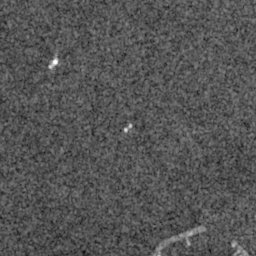
\includegraphics[width=0.38\textwidth]{detection_kish} &
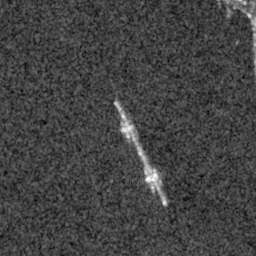
\includegraphics[width=0.38\textwidth]{persistent_kharg_jetty} \\
\small (الف) آشکارسازی مدل نزدیک کیش & \small (ب) اسکله نفتی خارک \\[4pt]
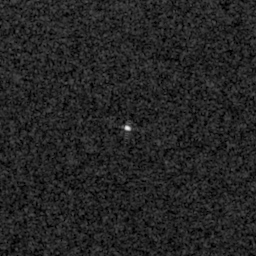
\includegraphics[width=0.38\textwidth]{persistent_assaluyeh} &
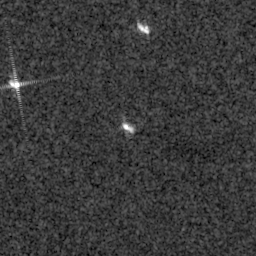
\includegraphics[width=0.38\textwidth]{persistent_bushehr} \\
\small (ج) پژواک نقطه‌ای پایدار نزدیک عسلویه & \small (د) پژواک‌های پایدار نزدیک بوشهر \\
\end{tabular}
\caption[برش‌های راداری آشکارسازی‌ها]{برش‌های راداری آشکارسازی‌ها در کنسول (قطبش \lr{VV}، شمال بالا، پهنای
\LRE{2٫56} کیلومتر، آشکارسازی در مرکز). (ب) تا (د) نقطه‌هایی‌اند که مدل در گذرهای بسیار در
آن‌ها چیزی می‌یابد؛ \lr{GFW} آن‌ها را سازه می‌شمارد و گزارش نمی‌کند.}
\label{fig:chips}
\end{figure}

قاعده نقطه پایدار (بخش~\ref{sec:persistence}) روی ۲۲۵ گذر-محدوده بایگانی \LRE{44} نقطه یافت.
نقاب کردن این نقطه‌ها روی گذرهای سپتامبر ۲۰۲۶ دقت مدل دور از ساحل ایران را از
\persistPrecisionBefore{} به \persistPrecisionAfter{} رساند، بی‌آنکه بازیابی کم شود
(جدول~\ref{tab:persistence}). اثر کوچک است: تنها حدود \LRE{6}٪ هشدارهای نادرست حذف شد، چون
بیشتر نقطه‌های تکرارشونده ۲۰۲۶ در بایگانی ۲۰۲۴ و ۲۰۲۵ نبودند. نقطه پایدار از گذرهای اخیر
باید ساخته شود؛ کنسول این آشکارسازی‌ها را علامت می‌زند و پنهان نمی‌کند.

\begin{table}[htbp]
\centering
\small
\begin{adjustbox}{max width=\textwidth}
\begin{tabular}{lcccc}
\toprule
مجموعه & امتیازدهی & دقت & بازیابی & \lr{F1} \\
\midrule
امارات، سپتامبر ۲۰۲۶ & استاندارد & \LRE{0٫591} ← \LRE{0٫594} & \LRE{0٫924} ← \LRE{0٫923} & \LRE{0٫721} ← \LRE{0٫723} \\
 & دور از ساحل & \LRE{0٫591} ← \LRE{0٫595} & \LRE{0٫924} ← \LRE{0٫924} & \LRE{0٫721} ← \LRE{0٫724} \\
ایران، سپتامبر ۲۰۲۶ & استاندارد & \LRE{0٫499} ← \LRE{0٫516} & \LRE{0٫905} ← \LRE{0٫905} & \LRE{0٫644} ← \LRE{0٫657} \\
 & دور از ساحل & \LRE{0٫509} ← \LRE{0٫523} & \LRE{0٫909} ← \LRE{0٫909} & \LRE{0٫652} ← \LRE{0٫664} \\
\bottomrule
\end{tabular}
\end{adjustbox}
\caption[اثر نقاب نقطه‌های پایدار]{اثر نقاب «نقطه‌های پایدار» (ساخته‌شده از گذرهای \lr{S1A} پیش از تیر ۱۴۰۵) روی گذرهای سپتامبر ۲۰۲۶، جداشده در زمان: پیش ← پس از حذف آشکارسازی‌های نزدیک نقطه‌ها؛ مرجع \lr{GFW} دست‌نخورده می‌ماند. «دور از ساحل»: خانه‌های بیش از ۱ کیلومتر از خشکی.}
\label{tab:persistence}
\end{table}


\section{نامزدهای شناور تاریک}
تلفیق خانه-ساعت (بخش~\ref{sec:fusion}) روی همه گذرهای سنجیده اجرا شد
(جدول~\ref{tab:dark}). روی گذرهای آزمون \darkUaeTest{} آشکارسازی‌های نگه‌داشته تاریک بودند، با
بیشترین نرخ در ناحیه هرمز. تلفیق ما با تطبیق خود \lr{GFW} سازگار است: از آشکارسازی‌هایی که
\lr{GFW} نیز بی‌\lr{AIS} می‌داند \LRE{36}٪ (\LRE{70} از \LRE{196}) تاریک شدند، و از آشکارسازی‌هایی
که \lr{GFW} با \lr{AIS} تطبیق داده تنها \LRE{2٫1}٪ (\LRE{74} از \LRE{3٬600}). نرخ تاریک با
بزرگ‌تر کردن حاشیه دروازه به‌سرعت کم می‌شود (شکل~\ref{fig:margin})؛ نامزدهایی که با حاشیه ۲
کیلومتر هم تاریک می‌مانند، اطمینان «زیاد» می‌گیرند.

\begin{table}[htbp]
\centering
\small
\begin{adjustbox}{max width=\textwidth}
\begin{tabular}{lccccc}
\toprule
مجموعه & گذر-محدوده & آشکارسازی نگه‌داشته & نرخ تاریک & بازه ۹۵٪ & داخلی / هرمز / عمان (٪) \\
\midrule
اعتبارسنجی & \LRE{25} & \LRE{1٬288} & \LRE{4٫0}٪ & \LRE{2٫6} تا \LRE{5٫8} & \LRE{6٫5} / \LRE{9٫2} / \LRE{2٫2} \\
آزمون & \LRE{92} & \LRE{4٬747} & \LRE{4٫0}٪ & \LRE{3٫2} تا \LRE{5٫3} & \LRE{7٫0} / \LRE{16٫8} / \LRE{1٫8} \\
\lr{S1A} ۲۰۲۶ & \LRE{21} & \LRE{1٬001} & \LRE{27٫8}٪ & \LRE{4٫7} تا \LRE{61٫3} & \LRE{27٫3} / \LRE{16٫7} / \LRE{28٫5} \\
\lr{S1C/D} & \LRE{42} & \LRE{2٬483} & \LRE{7٫9}٪ & \LRE{6٫3} تا \LRE{9٫7} & \LRE{18٫4} / \LRE{90٫9} / \LRE{5٫4} \\
\bottomrule
\end{tabular}
\end{adjustbox}
\caption[نرخ نامزد شناور تاریک]{نرخ نامزد شناور تاریک (تلفیق خانه-ساعت با حضور ساعتی \lr{AIS} از \lr{GFW}، حاشیه صفر متر که روی اعتبارسنجی برگزیده شد). اعتبارسنجی و آزمون: \lr{Sentinel-1A} ۲۰۲۴–۲۰۲۵؛ \lr{S1A} ۲۰۲۶: نیمه نخست ۲۰۲۶؛ \lr{S1C/D}: \lr{Sentinel-1C/1D} سپتامبر ۲۰۲۶. ستون آخر: خلیج داخلی، تنگه هرمز و دریای عمان. بازه‌ها با بوت‌استرپ روی برداشت‌ها.}
\label{tab:dark}
\end{table}


\begin{figure}[htbp]
\centering
\begin{tikzpicture}
\begin{axis}[
  width=0.8\textwidth, height=6cm,
  xmin=0, xmax=6, ymin=0, ymax=8.5,
  xtick={0,1,2,3,4,5,6},
  xticklabels={0, 250, 500, 1000, 2000, 5000, 10000},
  xlabel={\rl{حاشیه دروازه (متر)}}, ylabel={\rl{نرخ تاریک (٪)}},
  legend pos=north east, legend cell align=right,
  grid=major, grid style={gray!25},
]
\addplot[blue!70!black, thick, mark=*] table[x expr=\coordindex, y=test] {../data/dark_margin.csv};
\addlegendentry{\rl{آزمون \lr{S1A} ۲۰۲۴–۲۰۲۵}}
\addplot[orange!80!black, thick, mark=square*] table[x expr=\coordindex, y=s1cd] {../data/dark_margin.csv};
\addlegendentry{\rl{\lr{S1C/S1D} سپتامبر ۲۰۲۶}}
\end{axis}
\end{tikzpicture}
\caption[نرخ تاریک بر حسب حاشیه دروازه]{نرخ نامزد تاریک بر حسب حاشیه دروازه. حاشیه کاری (صفر متر) روی اعتبارسنجی برگزیده
شد.}
\label{fig:margin}
\end{figure}

نرخ نیمه نخست ۲۰۲۶ (\darkUaeEarly{}، با بازه‌ای بسیار پهن) از بقیه جداست: در ژانویه و فوریه
\LRE{3٫2}٪ و از مارس تا ژوئن \LRE{49}٪ بود. شکل~\ref{fig:aistrend} دلیل را نشان می‌دهد: از مارس
۲۰۲۶ ساعت-شناورهای حضور \lr{AIS} در خلیج فارس تقریباً نصف شد و سهم آشکارسازی‌های راداری
\lr{GFW} که با \lr{AIS} تطبیق می‌یابند هم‌زمان افتاد، در حالی که شمار آشکارسازی‌های راداری
تقریباً ثابت ماند. پس شناورها در دریا بودند ولی \lr{AIS} آن‌ها دیده نمی‌شد. نرخ تاریک در این دوره بیش
از رفتار شناورها، از دست رفتن پوشش \lr{AIS} را می‌سنجد؛ اخلال گسترده \lr{GNSS} در منطقه در
۲۰۲۵ و ۲۰۲۶ یک توضیح ممکن است که در این پژوهش آزموده نشد.

\begin{figure}[htbp]
\centering
\begin{tikzpicture}
\begin{axis}[
  width=0.95\textwidth, height=5.5cm,
  xmin=0, xmax=32, ymin=0, ymax=0.85,
  xtick={0,6,12,18,24,30},
  xticklabels={\lr{2024-01}, \lr{2024-07}, \lr{2025-01}, \lr{2025-07}, \lr{2026-01}, \lr{2026-07}},
  tick label style={font=\footnotesize},
  ylabel={\rl{سهم تطبیق‌یافته با \lr{AIS}}},
  legend pos=south west, legend cell align=right,
  grid=major, grid style={gray!25},
]
\addplot[blue!70!black, thick, mark=*, mark size=1pt] table[x=i, y=west] {../data/ais_trend.csv};
\addlegendentry{\rl{غرب ۵۶ درجه شرقی}}
\addplot[orange!80!black, thick, dashed, mark=square*, mark size=1pt] table[x=i, y=east] {../data/ais_trend.csv};
\addlegendentry{\rl{شرق ۵۶ درجه شرقی}}
\end{axis}
\end{tikzpicture}

\begin{tikzpicture}
\begin{axis}[
  width=0.95\textwidth, height=4.5cm,
  xmin=0, xmax=32, ymin=0, ymax=170,
  xtick={0,6,12,18,24,30},
  xticklabels={\lr{2024-01}, \lr{2024-07}, \lr{2025-01}, \lr{2025-07}, \lr{2026-01}, \lr{2026-07}},
  tick label style={font=\footnotesize},
  ylabel={\rl{هزار ساعت-شناور در روز}},
  grid=major, grid style={gray!25},
]
\addplot[teal, thick, mark=*, mark size=1pt] table[x=i, y=hours] {../data/ais_trend.csv};
\end{axis}
\end{tikzpicture}
\caption[روند حضور \lr{AIS} در خلیج فارس]{بالا: سهم آشکارسازی‌های راداری \lr{GFW} در خلیج فارس که با \lr{AIS} تطبیق یافته‌اند،
ماهانه. افت شرق از اکتبر ۲۰۲۵ خطای گذر \LRE{02:07} \lr{GFW} است؛ افت هر دو از مارس ۲۰۲۶ واقعی است.
پایین: حضور \lr{AIS} (ساعت-شناور در روز).}
\label{fig:aistrend}
\end{figure}

در ساحل ایران، روی تازه‌ترین گذری که حضور \lr{AIS} آن منتشر شده بود (۲۵ تا ۳۰ سپتامبر ۲۰۲۶)،
\LRE{109} آشکارسازی به دست آمد که \LRE{90} از پالایه‌ها گذشتند و \LRE{56} نامزد تاریک شدند:
بندرعباس ۳۳، بوشهر ۱۲، لارک/هرمز ۷، خارک ۲، کیش ۱، عسلویه ۱ و جاسک صفر (اطمینان زیاد ۱۶،
متوسط ۲۸، کم ۱۲). \lr{GFW} در خانه \LRE{32} نامزد آشکارسازی بدون \lr{AIS} دارد، در \LRE{19} خانه
چیزی ندارد و \LRE{5} نامزد را با \lr{AIS} تطبیق داده است. \LRE{24} نامزد در نقطه‌هایی‌اند که
در دست‌کم سه گذر دیگر نیز آشکارسازی داشته‌اند و ممکن است سازه یا شناور لنگرانداخته باشند.
در شش محدوده از هفت، شمار شناورهای تطبیق‌یافته \lr{GFW} برای داوری درباره کامل بودن حضور
\lr{AIS} کافی نبود؛ پس این شمارش‌ها نامزدند، نه یافته.

\section{کارایی}
روی پردازنده رایانه همراه این پژوهش (\lr{Ryzen 7 3700U}، بدون \lr{GPU})، اجرای مدل روی پنجره
\benchWindow{}$\times$\benchWindow{} پیکسلی یک محدوده ۲۰ کیلومتری به‌طور میانه \benchSeconds{} ثانیه
طول کشید، با بیشینه حافظه \benchMemory{} مگابایت. میانگین زمان مدل روی گذرهای واقعی آزمون
\testModelSeconds{} ثانیه بود (آبراه هرمز ۴۰ کیلومتری حدود چهار برابر یک محدوده ۲۰ کیلومتری
است). در اجرای ساحل ایران، هر محدوده از جست‌وجو تا ذخیره حدود ۳۰ تا ۴۰ ثانیه طول کشید و
هر درخواست حضور \lr{AIS} از \lr{GFW} حدود ۲۰ ثانیه؛ پس مدل تنگنای سامانه نیست.
